% ============================================================
% PAPIT — Project Proposal
% NeurIPS 2024 format
%
% REQUIRED: Download neurips_2024.sty from:
%   https://media.neurips.cc/Conferences/NeurIPS2024/Styles.zip
% Place neurips_2024.sty in the same directory as this file.
% ============================================================

\documentclass{article}
\usepackage[final]{neurips_2024}
\makeatletter
\renewcommand{\@noticestring}{}   % remove "37th Conference on NeurIPS..." footer
\makeatother

\usepackage[utf8]{inputenc}
\usepackage[T1]{fontenc}
\usepackage{hyperref}
\usepackage{booktabs}
\usepackage{tabularx}
\usepackage{amsmath}
\usepackage{microtype}
\usepackage{xcolor}
\usepackage{tikz}
\usetikzlibrary{arrows.meta, positioning, fit, backgrounds, calc}

% --- Color palette ---
\definecolor{cblue}{RGB}{214,234,248}   % Stage 1
\definecolor{cred}{RGB}{250,219,216}    % Stage 2
\definecolor{cgreen}{RGB}{213,245,227}  % Stage 3
\definecolor{cgray}{RGB}{240,240,240}   % I/O nodes

% ============================================================

\title{PAPIT: Prompt-Aware Pruning for Image Tokens \\
       in Efficient Multimodal Inference}

\author{%
  Chao Hsuan Ho \\
  \small\texttt{ch218@rice.edu}
  \And
  Heng Jui Hsu \\
  \small\texttt{hh83@rice.edu}
  \And
  Kerstin Sun \\
  \small\texttt{ks256@rice.edu}
}

\begin{document}
\maketitle
\vspace{-3.0em}

% ============================================================
\section*{Motivation}
% ============================================================
\vspace{-0.1em}
Multimodal Large Language Models (MLLMs) such as LLaVA tokenize images
into hundreds of visual patch tokens via a Vision Transformer (ViT).
The majority of these tokens are task-irrelevant given the user's
query — e.g., background scenery when the task is \emph{``count the fingers.''}
Standard \emph{global pruning} discards tokens without regard to the
current query, risking the loss of semantically critical patches.

We propose \textbf{PAPIT} (\textbf{P}rompt-\textbf{A}ware \textbf{P}runing for \textbf{I}mage \textbf{T}okens), a prompt-aware visual token pruning
framework that dynamically selects patches by computing cross-modal
cosine similarity between a CLIP text embedding and each visual patch
token. Only the top-$k$ most relevant tokens are retained, reducing
computational cost (FLOPs, latency) while preserving task accuracy.
Spatial anchoring maintains positional structure before the
pruned tokens are passed to LLaVA for final inference.

% ============================================================
\section*{System Diagram}
% ============================================================

\begin{center}
\resizebox{\textwidth}{!}{%
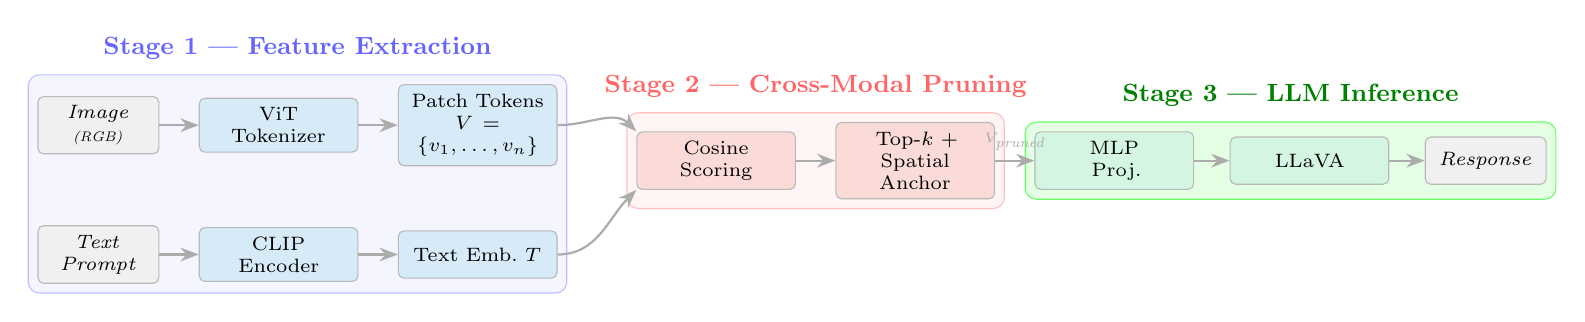
\begin{tikzpicture}[
  node distance = 0.40cm and 0.50cm,
  box/.style    = {rectangle, rounded corners=2pt, draw=gray!55,
                   fill=#1, text width=1.78cm, align=center,
                   minimum height=0.60cm, font=\scriptsize},
  iobox/.style  = {rectangle, rounded corners=2pt, draw=gray!55,
                   fill=cgray, text width=1.30cm, align=center,
                   minimum height=0.60cm, font=\scriptsize\itshape},
  arr/.style    = {-Stealth, thick, gray!65},
  stglbl/.style = {font=\small\bfseries},
  sublbl/.style = {font=\tiny\itshape},
]

%% --- I/O ---
\node[iobox]                      (img)   {Image\\{\tiny(RGB)}};
\node[iobox, below=0.90cm of img] (txt)   {Text Prompt};

%% --- Stage 1 ---
\node[box=cblue, right=of img]   (vit)   {ViT\\Tokenizer};
\node[box=cblue, right=of txt]   (clip)  {CLIP\\Encoder};
\node[box=cblue, right=of vit]   (vtok)  {Patch Tokens\\$V\!=\!\{v_1,\ldots,v_n\}$};
\node[box=cblue, right=of clip]  (temb)  {Text Emb.\ $T$};

%% --- Stage 2 ---
\node[box=cred,  right=1.0cm of vtok, yshift=-0.45cm] (score) {Cosine\\Scoring};
\node[box=cred,  right=0.50cm of score]                (topk)  {Top-$k$ +\\Spatial Anchor};

%% --- Stage 3 ---
\node[box=cgreen, right=0.50cm of topk]   (mlp)   {MLP\\Proj.};
\node[box=cgreen, right=0.45cm of mlp]    (llava)  {LLaVA};
\node[iobox,      right=0.45cm of llava]  (out)   {Response};

%% --- Arrows ---
\draw[arr] (img)  -- (vit);
\draw[arr] (vit)  -- (vtok);
\draw[arr] (txt)  -- (clip);
\draw[arr] (clip) -- (temb);
\draw[arr] (vtok.east) to[out=0,in=135] (score.north west);
\draw[arr] (temb.east) to[out=0,in=225] (score.south west);
\draw[arr] (score) -- (topk);
\draw[arr] (topk)  -- node[above, sublbl]{$V_{\text{pruned}}$} (mlp);

\draw[arr] (mlp)   -- (llava);
\draw[arr] (llava) -- (out);

%% --- Stage bounding boxes ---
\begin{pgfonlayer}{background}
  \node[draw=blue!25, fill=blue!4, rounded corners=4pt,
        fit=(img)(vit)(vtok)(txt)(clip)(temb),
        label={[stglbl, blue!60, yshift=2pt]above:%
               Stage 1 — Feature Extraction}] {};
  \node[draw=red!25, fill=red!4, rounded corners=4pt,
        fit=(score)(topk),
        label={[stglbl, red!60, yshift=2pt]above:%
               Stage 2 — Cross-Modal Pruning}] {};
  \node[draw=green!60, fill=green!10, rounded corners=4pt,
        fit=(mlp)(llava)(out),
        label={[stglbl, green!50!black, yshift=2pt]above:%
               Stage 3 — LLM Inference}] {};
\end{pgfonlayer}

\end{tikzpicture}}
\end{center}

\vspace{-0.2em}

% \noindent\textbf{Stage 1 — Feature Extraction.}
% A ViT tokenizes the input image into $n$ patch tokens
% $V = \{v_1,\ldots,v_n\}$.
% In parallel, the CLIP text encoder maps the user's prompt to a
% text embedding $T$ in the same latent space.

% \smallskip
% \noindent\textbf{Stage 2 — Cross-Modal Pruning.}
% Cosine similarity $s_i = \langle T,\, v_i \rangle / (\|T\|\|v_i\|)$
% is computed for every patch, producing a saliency map over the image grid.
% Top-$k$ selection retains the most prompt-relevant patches;
% spatial anchoring encodes their original grid positions before
% re-packing into the reduced set $V_{\text{pruned}}$.

% \smallskip
% \noindent\textbf{Stage 3 — LLM Inference.}
% $V_{\text{pruned}}$ is projected into LLaVA's embedding space via a
% lightweight MLP adapter and passed through LLaVA for final
% response generation.

% ============================================================
\section*{Evaluation Plan}
% ============================================================

We compare PAPIT against (i) an unpruned LLaVA baseline and
(ii) a global random-pruning baseline at matched retention ratios.

\vspace{0.4em}
\begin{tabularx}{\textwidth}{@{}llX@{}}
\toprule
\textbf{Dataset} & \textbf{Rationale} & \textbf{Metrics} \\
\midrule
GQA      & Complex spatial \& semantic reasoning
         & VQA accuracy, FLOPs, latency \\
VQA~v2   & Standard benchmark; broad comparison base
         & VQA accuracy, token retention rate \\
TextVQA  & Text in images: small but query-critical patches
         & VQA accuracy, patch recall on text regions \\
\bottomrule
\end{tabularx}
\vspace{0.3em}

We sweep the retention ratio $k \in \{25\%,\,50\%,\,75\%\}$ of $n$
and report the \textbf{accuracy–efficiency Pareto curve},
quantifying how much task performance is preserved per unit of
computational saving relative to both baselines.

% ============================================================
\section*{Future Work}
% ============================================================

As an optional extension, we will add a \textbf{Risk Awareness module}:
a safety prototype matcher that \emph{overrides} efficiency-driven pruning
to retain safety-critical patches (e.g., hazard signs, pedestrians) and
neutralize instruction-laden patches embedded in jailbreak images —
decoupling \emph{task relevance} from \emph{safety relevance}.

\end{document}
